$subject$=Физические основы компьютерных \\ и сетевых технологий
$teacher$=Лекции Герта А. В.
$date$=17.02.2025

\section{Лекция 2. Теорема Гаусса для магнитного поля}

В электростатике было введено понятие потока вектора напряженности электрического поля. Аналлогичное понятие
можно ввести для магнитного поля. 

\Def Потоком вектора магнитной индукции (или магнитным потоком) через элемент
площади $dS$ называется скалярная величина, равная $d\Phi = [\vec{B}, d\vec{S}] = B dS \cos \alpha = B_n dS$

Полный магнитный поток через поверхность $S$ равен сумме магнитных потоков через все элементы поверхности:

\[\Phi = \int_S [\vec{B}, d\vec{S}]\]

Теорема Гаусса для вектора индукции магнитного поля: поток вектора магнитной индукции сквозь произвольную замкнутую
поверхность равен нулю:

\[\oint_S [\vec{B}, d\vec{S}] = 0, \quad \mathrm{div}\vec{B} = 0\]

Эта теорема отражает факт непрерывности силовых линий магнитного поля, то есть отсутствия \enquote{магнитных зарядов}, 
на которых бы начинались или заканчивались линии магнитной индукции

Так как линии вектора индукции магнитного поля не имеют ни начала, ни конца, то число силовых линий, входящих в 
ограниченную замкнутую поверхность, равно числу выходящих из нее

Пусть магнитное поле создано бесконечно длинным прямолинейным проводником с током. Рассчитаем циркуляцию вектора
индукции магнитного поля по произвольному замкнутому контуру, охватывающему проводником

\[\oint_L [\vec{B}, d\vec{l}] = \oint_L Bdl \cos\alpha\]

\[dl \cos \alpha = r d\varphi, B = \frac{\mu_0 I}{2\pi r} \Longrightarrow \oint_L [\vec{B}, d\vec{l}] = \frac{\mu_0 I}{2\pi} \oint_L d\varphi = \mu_0 I\]

Получаем теорему о циркуляции вектора магнитной индукции: 

\begin{MyTheorem}
    Циркуляция вектора магнитной индукции по произвольному замкнутому
    контуру равна произведению магнитной постоянной на алгебраическую сумму токов, охватываемых этим контуром (или пронизывающих поверхность, опирающуюся на этот контур):

    \[\oint_L [\vec{B}, d\vec{l}] = \mu_0 \sum_k I_k\]
\end{MyTheorem}

При вычислении суммы токов нужно учитывать знаки: положительными считаются те токи, направление которых связано с направлением обхода
контура правилом правого винта, отрицательными - токи противоположного направления

Если контур в проводящей среде с непрерывным распределением тока, то $\oint_L [\vec{B}, d\vec{l}] = \mu_0 \int_S [\vec{j}, d\vec{S}]$

По теореме Стокса: $\oint_L [\vec{B}, d\vec{l}] = \int_S [\mathrm{rot}\vec{B}, d\vec{S}] = \mu_0 \int_S [\vec{j}, d\vec{S}]$

Таким образом, $\mathrm{rot}\vec{B} = \mu_0 \vec{j}$


\Ex Найдем магнитное поле соленоида (катушки)

Возьмем контур $L_1$ (см. кривой рисуночек), в нем $\oint_{L_1} [\vec{B}, d\vec{l}] = (B_{23} - B_{41})l = 0 \Longrightarrow B_{23} = B_{41} = B_\text{внутри}$

В другом контур $L_2$ $\oint_{L_2} [\vec{B}, d\vec{l}] = B_\text{внутри} l = \mu_0 NI \Longrightarrow B_\text{внутри} = \mu_0 \frac{N}{l} I = \mu_0 n I$, где $n$ - плотность витков катушки на длину катушки

\begin{center}
    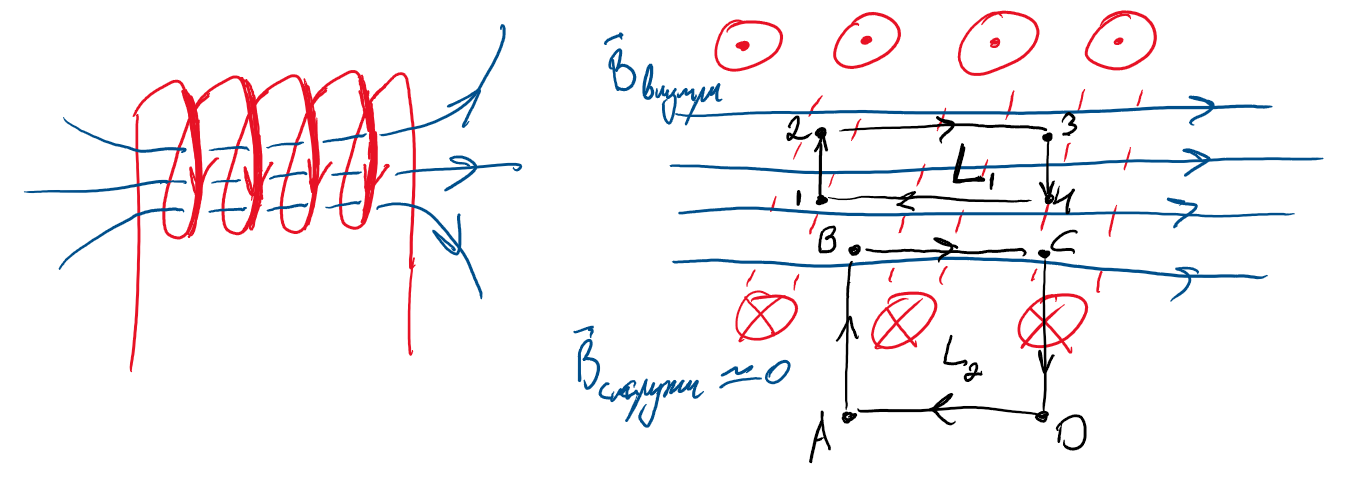
\includegraphics[width=15cm]{physics2/images/physics2_2025_02_17_1}
\end{center}

Получаем \fbox{$B = \mu_0 n I$} - поле катушки пропорционально плотности витков

\begin{minipage}{\textwidth}
    \begin{wrapfigure}{R}{0pt}
        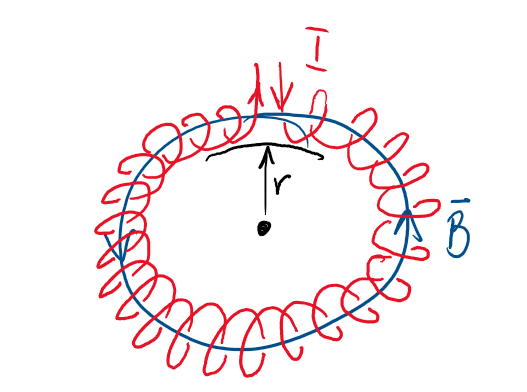
\includegraphics[width=6.3cm]{physics2/images/physics2_2025_02_17_2}
    \end{wrapfigure}

    \Ex Найдем поле тороида. Из соображений симметрии очевидно, что линии индукции - окружность, концентричные с тороидом. В качестве контура $L$ выберем окружность с радиусом $r$

    $\oint_L [\vec{B}, d\vec{l}] = B \cdot 2\pi r = \mu_0 N I \Longrightarrow$ \fbox{$B(r) = \frac{\mu_0 N I}{2\pi r}$}, 
    где $N$ - число витков

    Вектора магнитной индукции будут являться касательными к окружности, концентричной тороиду

\end{minipage}

\Ex Постоянный ток $I = 10$ А, течет по длинному прямому проводнику круглого сечения. Найти магнитный поток через одну
из половин осевого сечения проводника в расчете на один метр его длины.

\mediumvspace

Возьмем контур $L$ - окружность радиуса $r$, меньшего радиуса сечения проводника $R$. 
По теореме о циркуляции $\oint_L B(r) dr = \mu_0 I_\text{внутри}$. В силу симметрии считаем, что вектор $\vec B(r)$ равен по модулю на всем контуре $L$.
Тогда получаем $B(r) \cdot 2\pi r = \mu_0 I_\text{внутри} = \mu_0 j S = \mu_0 j \pi r^2 \Longrightarrow B(r) = \frac{\mu_0 I r}{2 \pi R^2}$

Тогда поток через половину осевого сечения равен $\frac{\Phi}{l} = \int_0^R B(r) dr = \int_0^R \frac{\mu_0 I r}{2\pi R^2} dr = $ \fbox{$\frac{\mu_0 I}{4 \pi}$} $ = 10^{-6} \frac{\text{Вб}}{\text{м}}$

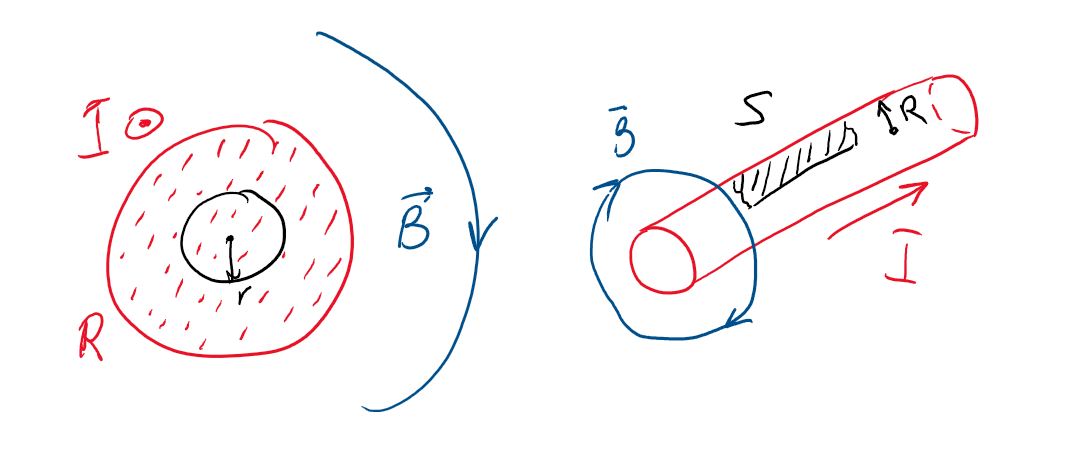
\includegraphics[width=15cm]{physics2/images/physics2_2025_02_17_3}

\begin{minipage}{\textwidth}
    \begin{wrapfigure}{R}{0pt}
        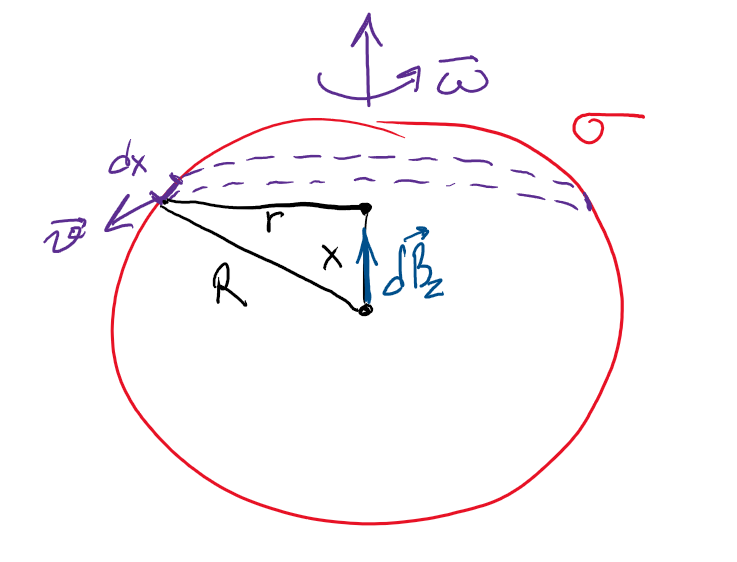
\includegraphics[width=6cm]{physics2/images/physics2_2025_02_17_4}
    \end{wrapfigure}

    \Ex Непроводящая сфера радиуса $R = 50$ мм, заряженная равномерно с поверхностной плотностью $\sigma = 10$ мкКл/м$^2$, 
    вращается с угловой скоростью $\omega = 70$ рад/с вокруг оси, проходящей через ее центр. Найти магнитную индукцию в центре сферы

    \mediumvspace

    Сделаем разбиение сферы на колечки высотой $dx$, длина каждой такой колечки равна $2\pi r$, где $r = \sqrt{R^2 - x^2}$.
    Его площадь $2\pi r dx$. Точка на кольце движется с линейной скоростью $v = \omega r$.
\end{minipage}

В силу симметрии вектор магнитной индукции $d\vec{B}$, производимый кольцом, параллелен оси $Oz$. 
Тогда $dB = \frac{\mu_0}{4\pi} \frac{q \cdot v}{R^2} = \frac{\mu_0}{4\pi} \frac{\sigma 2\pi r \cdot dx \cdot \omega r}{R^2} = 
\frac{\mu_0}{4\pi} \frac{\sigma 2\pi \omega (R^2 - x^2)}{R^2} dx$

В интеграле $B = \int_{-R}^R dB = \frac{\sigma \mu_0 \omega}{2} \int_{-R}^R \frac{(R^2 - x^2)}{R^2} dx = 
\frac{\sigma \mu_0 \omega}{2} \frac{(R^2 x - \frac{1}{3} x^3)}{R^2} \Big|_{-R}^R = 
\frac{\sigma \mu_0 \omega}{2} \frac{(R^2 x - \frac{1}{3} x^3)}{R^2} \Big|_{-R}^R = 
\frac{\sigma \mu_0 \omega}{2} \frac{4}{3} R = $ \fbox{$\frac{2}{3} \mu_0 R \omega \sigma$}


